\documentclass[letterpaper]{article} % DO NOT CHANGE THIS
\usepackage[submission]{aaai2027} % DO NOT CHANGE THIS
% The serif, sans-serif, and monospaced fonts are loaded automatically by
% aaai2027.sty (newtxtext, helvet, courier). DO NOT add \usepackage{times},
% \usepackage{helvet}, \usepackage{courier}, or any other font package.
\usepackage[hyphens]{url} % DO NOT CHANGE THIS
\usepackage{graphicx} % DO NOT CHANGE THIS
\urlstyle{rm} % DO NOT CHANGE THIS
\def\UrlFont{\rm} % DO NOT CHANGE THIS
\usepackage{natbib} % DO NOT CHANGE THIS AND DO NOT ADD ANY OPTIONS TO IT
\usepackage{caption} % DO NOT CHANGE THIS AND DO NOT ADD ANY OPTIONS TO IT
\frenchspacing % DO NOT CHANGE THIS

% --- Math / theorems / tables (compatible with aaai2027.sty) ---
\usepackage{amsmath,amssymb,amsthm}
\theoremstyle{plain}
\newtheorem{theorem}{Theorem}
\newtheorem{proposition}{Proposition}
\usepackage{booktabs}

\pdfinfo{
/TemplateVersion (2027.1)
}

\newcommand{\wcrit}{w_{\mathrm{crit}}}
\newcommand{\PT}{\mathrm{PT}}

\setcounter{secnumdepth}{0}

\title{Measuring the Coordination-Collapse Boundary in Policy-Gradient Cooperative MARL}

\author{
  Anonymous Submission
}
\affiliations{
  Paper under double-blind review
}

\begin{document}

\maketitle

% =======================================================================
\begin{abstract}
Cooperative multi-agent reinforcement learning (MARL) can collapse into a degenerate
\emph{lazy-agent} policy when reward centralization is too low, but the field describes this
failure only qualitatively. Our contribution is a way to measure it: a pre-registered collapse
definition and bootstrap confidence intervals that turn the failure into a critical
centralization $\wcrit$ with error bars. We then use the instrument to ask whether behavioral preferences move the
threshold, and find that they do: \emph{loss aversion} systematically shifts $\wcrit$ rightward, so
loss-averse agents need more centralization to coordinate. This effect is monotone in the
loss-aversion strength $\lambda$ and replicates in direction across four environment-algorithm
combinations; at the human range ($\lambda\!\approx\!3$) it adds $+0.089$ to the required
centralization net of curvature ($+0.188$ in isolation). We report what is robust (the boundary, and the direction of the loss-aversion
effect) separately from what is substrate-specific (the effect's magnitude and functional form),
and offer a supporting mean-field account at the level of sign, not magnitude. The pre-registered
protocol is a reusable instrument for measuring where a cooperative-MARL system collapses, and how far
behavioral bias moves that point.
\end{abstract}

% =======================================================================
\section{Introduction}
\label{sec:intro}

A team of learning agents sharing a task can fall into a trap their designers never intended:
instead of coordinating, every agent quietly defaults to inaction, and the team settles into a
stable, useless equilibrium: \emph{coordination collapse}, whose endpoint is the \emph{lazy-agent}
policy~\citep{liu2023lazy,peng2023curo}, an instance of the sequential social dilemma that arises
when private incentives drift from the collective good~\citep{leibo2017multi}. Whether a team falls
in is governed by one design dial, the \emph{reward centralization} $w\in[0,1]$: the share of each
agent's reward tied to the team's outcome rather than its own. Turn $w$ down and an agent's private performance
drowns out its contribution, so cooperating earns no learnable signal and the safe policy
wins. The field knows this only as a direction (\emph{more centralization
helps}~\citep{dmarl2025,liu2023lazy}) and stops there. \emph{Where}, in $w$, a working team
tips into collapse has not, to our knowledge, been measured. Our central question is therefore twofold: does
coordination collapse admit a \emph{measurable} critical centralization threshold, and do
behavioral preferences systematically shift it? The first half is a measurement problem (the
paper's primary contribution), and the second is a question the instrument then makes answerable. Prior work either mitigates the lazy-agent pathology without locating a boundary or sweeps
neighboring axes, and the closest phase-diagram studies place their critical points on
\emph{environmental} or opinion-dynamics axes rather than reward structure. None measures a
confidence-intervalled reward-centralization threshold, in gradient-trained cooperative policies,
that a behavioral bias then moves; we differentiate against the closest prior work below.

Pinning that number down matters now, because deployed agents are no longer neutral optimizers. In
automated replenishment, fraud review, and energy dispatch, learning agents absorb human preference
structure by construction: trained on human choices through preference-aligned objectives that are
themselves prospect-theoretic~\citep{ethayarajh2024kto}, or sharing the loop with human
operators~\citep{lalmohammed2025}. The sturdiest such regularity is \emph{loss aversion}: a loss
looms larger than an equal gain~\citep{kahneman1979,tversky1992}. Behavioral economics knows what
this does to one chooser but is silent on a \emph{group} learning to
coordinate~\citep{leibo2017multi,lowe2017multi}. A measured collapse boundary is the instrument that
question needs, extending the thin existing bridge between behavioral preferences and collective
learning dynamics to the prospect-theoretic preferences today's training pipelines instill.

We therefore build the ruler first, and treat it as the paper's central object. Following the
posture physics takes toward a phase boundary, we fix a binary collapse criterion in advance,
freeze it, fit $P(\mathrm{collapse}\mid w)$, and bootstrap confidence intervals on $\wcrit$.
(``Phase boundary'' is used in the empirical, learning-dynamics sense
of~\citet{yamaguchi2025,capannoli2026phase}, not as a thermodynamic-criticality claim.) Two design
choices keep the readings honest: we apply cumulative prospect theory (CPT) as a \emph{reward
transform} after blending rather than inside the update, so the optimizer is bit-identical across
conditions and any movement of $\wcrit$ is behavioral; and we re-measure at several horizons, since
a drifting threshold could pass for a constant. Our \emph{primary} contribution is
(i) a confidence-intervalled measurement of the coordination-collapse boundary in policy-gradient
cooperative MARL, with a reusable pre-registered protocol. Using that instrument, we then establish
three findings about behavioral bias: (ii) loss aversion shifts the boundary rightward, a direction
whose sign we fix a priori and confirm across four environment-algorithm combinations, with the
metastable horizon slide generalizing likewise; (iii) prospect theory's two components move it in
\emph{opposite} directions; and (iv) on a directed-flow substrate, a downstream loss-averse
\emph{minority} can set the boundary for the whole system. What is new is specific, and stated
against the closest prior work below: the measured, CI'd boundary and the component decomposition
against it, in gradient-trained neural policies.

% =======================================================================
\section{Related Work}
\label{sec:related}

\paragraph{Coordination collapse and credit assignment.}
Cooperative MARL, studied since independent $Q$-learning on shared
tasks~\citep{tan1993multi,busoniu2008comprehensive}, inherits the lazy-agent and
relative-overgeneralization failures in which agents abandon cooperation for a degenerate
policy~\citep{liu2023lazy,peng2023curo,tampuu2017multiagent}. The standard remedy is centralized
credit assignment under CTDE, a centralized critic or factorized value
function~\citep{lowe2017multi,yu2022surprising,sunehag2018vdn,rashid2018qmix,foerster2018counterfactual,son2019qtran};
related work ties the failure to
decentralized exploration~\citep{weng2026} or shows decentralized shaping cannot match centralized
baselines~\citep{dmarl2025}. This establishes \emph{that} centralization helps and \emph{how} to
implement it; none locates the threshold $\wcrit$ or gives it a confidence interval, the gap we
close, using $w$ as the dial rather than a fixed factorization.

\paragraph{Phase transitions in multi-agent learning.}
Treating collective learning as a dynamical system with critical points has
precedent: \citet{yamaguchi2025} build a phase diagram for independent Q-learning over
\emph{environmental} axes, \citet{capannoli2026phase} prove a metastable boundary in opinion
dynamics under a fixed update rule, and the mean-field programme for multi-agent
learning~\citep{barfuss2019deterministic,hu2019meanfield,hussain2025convergence} derives
Fokker--Planck descriptions of networked Q-learning. We share this statistical-physics posture but
differ in object, ours is a \emph{reward-structure} threshold with confidence intervals that a
\emph{behavioral} parameter moves, and use the mean-field machinery only to fix a sign.

\paragraph{Behavioral preferences in cooperative AI.}
A thin bridge connects human preference structure to collective learning dynamics:
\citet{hughes2018inequity} show inequity aversion improves cooperation within the cooperative-AI
agenda~\citep{dafoe2020open,hammond2025multiagent,barfuss2020caring}. Risk-sensitive RL optimizes
tail outcomes~\citep{qiu2021rmix,xie2023riskq,prashanth2014cvar,tamar2015optimizing}, distinct from
loss aversion, a reference-point asymmetry, and prospect theory has entered single-agent RL with
known calibration concerns~\citep{prashanth2016cumulative,rabin2000risk,tversky1992}. In the
multi-agent setting, \citet{mengesha2025} prove loss aversion shifts a tipping point in evolutionary
game theory over fixed strategies, and \citet{lalmohammed2025} bring CPT into cooperative MARL but
fold it into the update, entangling its components. We differ at the level of \emph{apparatus}:
rather than proposing another behavioral model, we build a measured boundary and use it as a common
instrument, the behavioral study is its first application, not the contribution.

% =======================================================================
\section{Preliminaries and Method}
\label{sec:method}

In cooperative MARL, $N$ agents share an environment and maximize a joint objective under
CTDE~\citep{lowe2017multi}; the reward-mixing weight $w\in[0,1]$ interpolates purely local
($w{=}0$) and purely global ($w{=}1$) reward. As $w\!\to\!0$ the cooperative signal is diluted
and agents collapse to the safe lazy policy~\citep{liu2023lazy,peng2023curo}. This $w$ is our
sole structural intervention; all else is held fixed, so any boundary shift is attributable to
$w$ and the behavioral parameters. Cumulative prospect theory~\citep{kahneman1979,tversky1992}
gives the value function $v(x)=x^\alpha$ for $x\ge0$ and $-\lambda(-x)^\beta$ for $x<0$, where
$\alpha,\beta\in(0,1]$ govern curvature and $\lambda>1$ is loss aversion
($\alpha{=}\beta{=}1,\lambda{=}1$ is linear utility). We apply it as a reward transform after
blending,
\begin{equation}
 r_i^{\PT}=v\!\left((1-w)\,r_i^{\mathrm{local}}+w\,r^{\mathrm{global}}\right),
 \label{eq:reward}
\end{equation}
the decisive difference from \citet{lalmohammed2025}, who fold CPT \emph{into} the
actor--critic update, entangling curvature with loss aversion and confounding any shift with a
change to the optimizer. Transforming only the scalar reward leaves the policy gradient
identical across conditions, so a measured shift is behavioral and the two channels dial
independently. We pre-registered the binary collapse label
$\mathbf{1}[\bar S<10\wedge\bar\pi\le-127.1]$ ($\bar S$ mean base-stock, $\bar\pi$ mean profit),
freezing it in version control before any analysis; the frozen label and its analysis code ship in
the anonymized supplementary code bundle so the pre-registration is verifiable at review time, with
the de-anonymized commit hash and public repository released on acceptance. It is robust to
$\pm20\%$ threshold perturbation (max $\Delta\wcrit=0.015$;
Supplement). For
each condition we fit $P(\mathrm{collapse}\mid w)=\sigma(b_0+b_1 w)$, estimate
$\wcrit=-b_0/b_1$ (the $w$ at which $P(\mathrm{collapse})=0.5$), and bootstrap its 95\% CI; steep
high-$\lambda$ cells use Firth penalized regression, whose $\wcrit$ agrees with the bootstrap
estimate to within $0.019$ at every $\lambda$, two independent estimators concur, so the boundary
locations are not an artifact of either fitting method.
The logistic midpoint is the natural transition point: collapse is a \emph{binary} per-run outcome,
so the sigmoid is its maximum-entropy model and $-b_0/b_1$ is the location parameter (the $w$ of
maximal uncertainty). The transition is empirically \emph{sharp}: collapse fractions rise from
near-zero to near-one within $\Delta w<0.3$, so this is the center of a narrow, well-identified
crossing, not an arbitrary cut through a gentle slope; we report its width $\Delta w$ alongside its
location. We use ``phase boundary'' in this empirical sense, not as a thermodynamic-criticality
claim. The decomposition compares three
conditions with identical environment and optimizer: \textbf{Null} ($\alpha{=}\beta{=}1,
\lambda{=}1$), \textbf{Curvature} ($\alpha{=}\beta{=}0.88,\lambda{=}1$), and \textbf{Loss
aversion} ($\alpha{=}\beta{=}0.88,\lambda>1$). The primary substrate is
\texttt{NetworkManagement-v1}~\citep{hubbs2020orgym}, a six-node multi-echelon inventory
network~\citep{oroojlooyjadid2022,gijsbrechts2022,marlim2023}; transfer environments are MPE
Cooperative Navigation~\citep{lowe2017multi} and Level-Based Foraging~\citep{christianos2020shared}.
We choose this over combat benchmarks such as SMAC~\citep{samvelyan2019smac} deliberately: measuring
how $w$ moves the boundary needs a sequential social dilemma with a directed resource flow, whereas
SMAC-style tasks couple spatial configuration and credit assignment with the quantity we isolate; we
then confirm the \emph{direction} on MPE and LBF to rule out a supply-chain artifact. Agents run
PPO~\citep{schulman2017ppo} via Stable-Baselines3~\citep{raffin2021sb3} and
PettingZoo/SuperSuit~\citep{terry2021pettingzoo,terry2020supersuit} (20 seeds/condition, 1{,}524
runs). Full setup is in the Supplement.

% =======================================================================
\section{The Boundary and Its Behavioral Shift}
\label{sec:results}

\paragraph{A sharp, metastable boundary.}
Collapse is a sharp logistic transition in $w$, not a gradual decay: at 300k steps
$\wcrit=0.666$ $[0.635,0.694]$ (transition width $\Delta w=0.199$, $p=3.2\times10^{-7}$), with
collapse fractions rising from near-zero to near-one within $\Delta w<0.3$
(Figure~\ref{fig:boundary}a). The boundary is not a constant but a \emph{metastable} threshold that
slides left with the training horizon, and across four matched risk-neutral horizons
($\wcrit=0.822,0.666,0.622,0.573$ at $150\mathrm{k},300\mathrm{k},450\mathrm{k},900\mathrm{k}$) the
slide is \emph{log-linear in $T$}: $\wcrit=2.44-0.138\ln T$ (RMSE $0.027$; all four CIs of width
${\le}0.04$; Figure~\ref{fig:boundary}b). This log-linear form is \emph{consistent with} metastable
escape (a Kramers-type first-passage picture, developed below): each doubling of the budget
buys a fixed $\approx0.10$ leftward shift in $w$, so the boundary keeps falling below the longest
measured point
($0.573$ at 900k), extrapolating the law to $2\mathrm{M}$ steps gives $\wcrit\approx0.44$. Collapse
at intermediate $w$ is therefore the metastable \emph{approach} to the deterministic floor
$\wcrit^0=c/(c+g)$ the mechanism derives below, escapable with more training, not
absorbing; we treat the floor's exact value as below the measured range rather than extrapolating
the log-linear form to an (unphysical) zero crossing. This horizon dependence does not make $\wcrit$
arbitrary: a log-linear slide is the signature of a metastable, not ill-defined, threshold, at any
fixed budget it is a well-defined number, and it quantifies a second design axis, the rate at which
extra training rescues a sub-boundary policy (trading compute against centralization). The slide is not a supply-chain artifact either: under centralized-critic MAPPO it recurs
in both transfer environments, on MPE $\wcrit$ falls $0.82\to0.68$ as the horizon grows
$2\mathrm{M}\to8\mathrm{M}$, and on Level-Based Foraging
$0.33\to0.20$ over $1\mathrm{M}\to4\mathrm{M}$, both with non-overlapping intervals. A
basin-control experiment rules out initialization as the driver: within-$w$ correlations between
initial and converged base-stock are near zero ($-0.11$ to $-0.38$), so the collapse label does not
track where agents start (Supplement).

\paragraph{Loss aversion raises the boundary; curvature lowers it.}
Against a single canonical null, $\wcrit^{\mathrm{null}}=0.666$ $[0.635,0.694]$, independently
reproduced at $0.685$ by a dedicated experiment (every other null-like number is a labeled
offset, not a separate baseline), we sweep $\lambda\in\{1,\dots,7\}$ ($\alpha{=}\beta{=}0.88$,
300k). The boundary rises monotonically with loss aversion, $\{0.586,0.715,0.774,0.806,0.825,
0.835,0.852\}$, then saturates near $0.85$ with clear headroom to the $w{=}1$ ceiling, so the
plateau is behavioral, not a ceiling artifact (Figure~\ref{fig:decomposition},
Table~\ref{tab:decomposition}); the endpoints are non-overlapping by $0.221$. Curvature acts in
the \emph{opposite} direction, \emph{lowering} $\wcrit$ to $0.586$ ($-0.100$ $[-0.172,-0.033]$
vs.\ the null), that a single ``risk-averse'' psychology pulls the boundary in opposite directions
is the first of two surprises, visible only against a calibrated null.

\paragraph{Two ways to count the loss-aversion effect.}
The magnitude depends on the baseline, and we report both (Table~\ref{tab:decomposition}). Against
the \emph{linear null} ($0.685$) the combined CPT shift is $+0.089$ at $\lambda{=}3$ and $+0.166$ at
$\lambda{=}7$, but this nets loss aversion against curvature's $-0.100$; the \emph{pure
loss-aversion increment} against the curvature baseline ($0.586$) (the correct isolate) is larger,
$+0.188$ and $+0.265$ (reconciled by the offset, $-0.100+0.265\approx0.166$). Throughout, ``the
loss-aversion effect'' means the increment over the curvature baseline; the net-vs-null figure is
the deployment total. The full sweep is tracked by a one-parameter, theory-bounded affine law
(derived below) to RMSE $0.014$, and a finer $w\in\{0.80,0.90\}$ grid tightens the steep
$\lambda{\geq}5$ cells to CI widths $\approx0.03$ (half those from a single $w{=}0.85$ cell).

\begin{figure}[t]
 \centering
 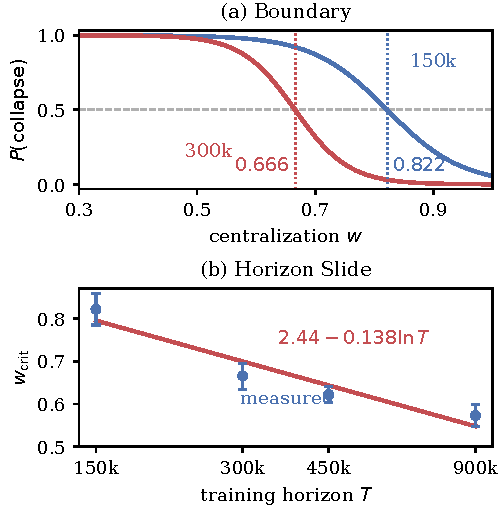
\includegraphics[width=\columnwidth]{Figures/boundary_metastability}
 \caption{(a)~Collapse is a sharp logistic transition in $w$; the boundary sharpens and slides
  left from 150k to 300k steps. (b)~Across four matched risk-neutral horizons (20 seeds each,
  all CIs of width ${\le}0.04$) $\wcrit$ falls \emph{log-linearly} in $T$, $\wcrit=2.44-0.138\ln
  T$ (RMSE $0.027$), consistent with the metastable escape the mechanism predicts.}
 \label{fig:boundary}
\end{figure}

\begin{figure}[t]
 \centering
 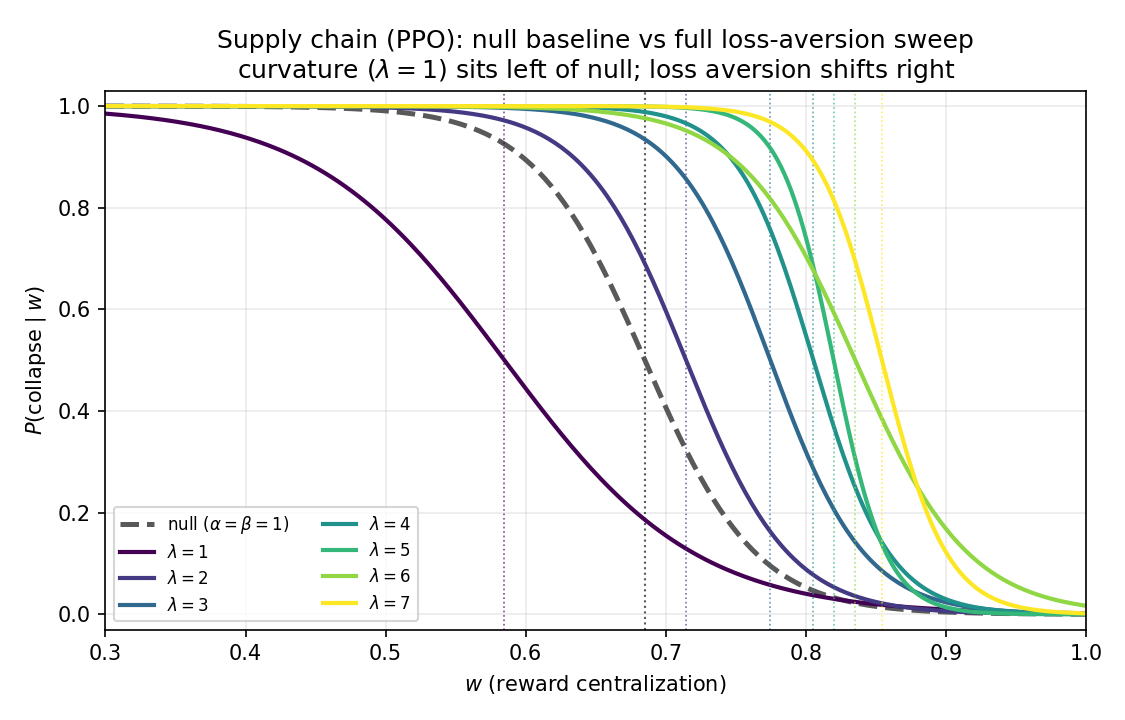
\includegraphics[width=0.92\columnwidth]{Figures/ppo_behavioral_full}
 \caption{Behavioral decomposition and full loss-aversion sweep (supply chain, PPO). Curves
  are Firth-fitted $P(\mathrm{collapse}\mid w)$; dotted lines mark $\wcrit$. Curvature
  ($\lambda{=}1$) sits \emph{left} of the null (easing coordination); loss aversion
  ($\lambda{=}2,\dots,7$) shifts $\wcrit$ \emph{right}, rising then saturating.}
 \label{fig:decomposition}
\end{figure}

\begin{table}[t]
\centering
\caption{Three-way decomposition of $\wcrit$. We report the effect both ways: net vs.\ the
linear null (combines curvature and loss aversion), and the pure loss-aversion increment vs.\
the curvature baseline ($0.586$). ``Sig.'' = difference CI excludes zero.}
\label{tab:decomposition}
{\setlength{\tabcolsep}{4.5pt}
\begin{tabular}{lccc}
\toprule
Condition & $\wcrit$ & vs.\ null & vs.\ curv. \\
\midrule
Null ($\lambda{=}1$) & 0.685 & -- & -- \\
Curvature ($\lambda{=}1$) & 0.586 & $-0.100^{\checkmark}$ & 0 \\
Loss av.\ $\lambda{=}3$ & 0.774 & $+0.089^{\checkmark}$ & $+0.188$ \\
Loss av.\ $\lambda{=}7$ & 0.852 & $+0.167^{\checkmark}$ & $+0.266$ \\
\bottomrule
\end{tabular}}
\end{table}

% =======================================================================
\section{A Mean-Field Mechanism Fixes the Sign}
\label{sec:mechanism}

The measurement above is the paper's contribution; this section adds a \emph{supporting} account of
why the boundary exists and which way each component moves it. It is deliberately modest, sign and
form, not magnitude, and not the basis of any empirical claim, so the results stand whether or not
the reader accepts it. Following mean-field treatments of multi-agent
learning~\citep{barfuss2019deterministic,hu2019meanfield,hussain2025convergence}, we model each
Gaussian-policy agent's mean action as a Langevin variable
$\mathrm{d}\mu_i=D(w)\,\mathrm{d}t+\sqrt{2\Theta(w)}\,\mathrm{d}W$ (details in the Supplement), with
drift $D$ and a centralization-weighted diffusion $\Theta$ into which partner exploration enters.
The replenishing regime makes an upstream node's inventory a local cost but a global benefit, giving
cooperative drift $D(w)=\eta[wg-(1-w)c]$. Escape from the lazy basin is
governed not by drift but by its ratio to gradient noise,
\begin{equation}
 \mathrm{SNR}(w)=\frac{D(w)}{\sqrt{\Theta(w)}}\gtrsim\kappa_c,
 \label{eq:snr}
\end{equation}
and the crossing defines $\wcrit$. Treating escape as a Kramers first-passage
problem~\citep{kramers1940brownian}, the noise-induced analogue of a saddle-node
bifurcation~\citep{strogatz1994nonlinear}, gives two expectations \emph{consistent with} the data:
collapse switches abruptly across $\wcrit$ and $\wcrit(T)$ falls as $T$ grows. It also makes a
\emph{falsifiable} prediction we test directly: raising exploration noise should raise $\wcrit$, but
only where that noise is the \emph{binding} term. An entropy ablation confirms this as a
\emph{dissociation} (Figure~\ref{fig:dissociation}): $\wcrit$ rises with the entropy coefficient on
the supply chain and LBF (sparse rewards, injected entropy dominates) but stays flat on MPE (dense
reward, high intrinsic exploration swamps the added term). The effect appears exactly where the
mechanism predicts and is \emph{absent} where it predicts none, a sharper test than uniform
replication, and the one prediction a skeptic cannot dismiss as single-substrate luck. The mechanism does \emph{not} deliver the value of
$\wcrit$: $c,g,\sigma,\kappa_c$ are calibrated, and two pre-registered probes to localize it from
the drift were inconclusive (survivor bias in the contested band; Supplement). The magnitude thus
stays calibrated; the mechanism's content is the sign and the form.

\begin{figure}[t]
 \centering
 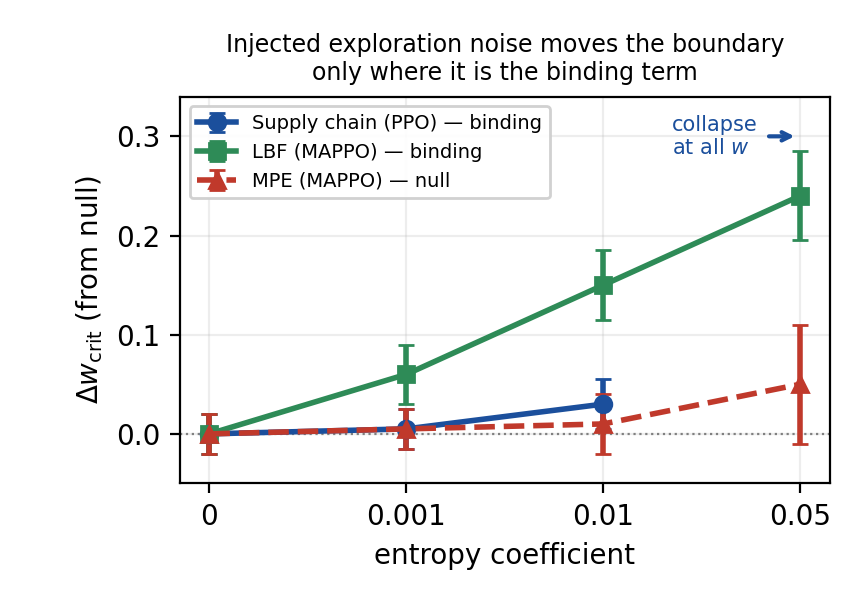
\includegraphics[width=0.82\columnwidth]{Figures/entropy_dissociation.png}
 \caption{Entropy-ablation dissociation. Injected exploration noise raises $\wcrit$ on the
  supply chain (PPO) and LBF (MAPPO), where it is the binding noise term, but leaves the MPE
  boundary flat (overlapping CIs), where dense-reward intrinsic exploration dominates, a
  prediction that correctly stays null is evidence of mechanism, not curve fitting.}
 \label{fig:dissociation}
\end{figure}

We are direct about the one place the account could be read as circular. The sign result below
assumes a payoff premise ($\partial_\lambda F<0$): by asymmetrically down-weighting gains against
losses, loss aversion biases the expected update toward the conservative lazy action, weakening the
cooperative drift and so the signal-to-noise ratio. We do \emph{not} take this on faith or
infer it from the outcome; we verify it independently with a finite-difference probe of the
substrate (Supplement), so the proposition's content is the non-trivial claim that this
\emph{locally} measured sign \emph{propagates} to the \emph{global} boundary through the intractable
noise, not the assumption that loss aversion hurts coordination.

\begin{proposition}[Sign propagation of the loss-aversion shift]\label{thm:sign}
Let the order parameter $x$ evolve as $\mathrm{d}x_t=F(x_t,w,\lambda)\,\mathrm{d}t+
\sqrt{\Sigma(x_t,N)}\,\mathrm{d}W_t$ with $\Sigma>0$, and \emph{assume the payoff premise}
$\partial_\lambda F<0$ on the escape interval, i.e.\ loss aversion scales only the loss domain
and so biases the drift toward the conservative action. Then $\partial_\lambda \wcrit^{\mathrm{Emp}}>0$.
\end{proposition}
\begin{proof}[Proof sketch]
The barrier to escape the lazy basin, $\Delta U=\int_{x^\ast_{\mathrm{lazy}}}^{x^\ast_{\mathrm{saddle}}}(-2F/\Sigma)\,\mathrm{d}z$, has $\partial_\lambda\Delta U>0$
pointwise, since $\Sigma>0$ and $\partial_\lambda F<0$ throughout, independent of the sign of
$F$: loss aversion steepens the drift toward the lazy state and raises the barrier. A higher
barrier lengthens escape ($\partial_\lambda\tau>0$) while $\partial_w F>0$ lowers it
($\partial_w\tau<0$); collapse is failure to escape within budget ($\tau>T$). The implicit
function theorem on $\tau(w,\lambda)=T$ gives $\mathrm{d}\wcrit^{\mathrm{Emp}}/
\mathrm{d}\lambda=-\partial_\lambda\tau/\partial_w\tau>0$. The magnitude depends on the
intractable $\Sigma$; the direction does not. The same argument with curvature's drift signs
reversed yields the opposite shift.
\end{proof}

We state this as a \emph{proposition}, not a theorem, because its force is conditional: it assumes
the payoff premise $\partial_\lambda F<0$ rather than deriving it from first principles. We verify
that premise directly on the substrate (a finite-difference probe confirms the loss-domain gradient
asymmetry that produces this conservative drift; Supplement), so the result's content is that this \emph{local}
sign propagates to the \emph{global} boundary regardless of the intractable noise $\Sigma$, which
is exactly what makes the direction (but not the magnitude) predictable. The two prospect-theory
components move the boundary through opposite channels of the same SNR, without fitting: curvature
($\alpha,\beta<1$) compresses gains and losses \emph{symmetrically}, lowering the diffusion
$\Theta$, raising the SNR, and so \emph{lowering} $\wcrit$; loss aversion acts
\emph{asymmetrically} on the drift, weakening $D$, lowering the SNR, and \emph{raising} it, matching
the measured $-0.100$ and $+0.265$ (Table~\ref{tab:decomposition}).

\paragraph{A theory-bounded law, tested out of sample.}
The same loss-domain split fixes the functional \emph{form}, not just the sign. Only the loss
domain scales with $\lambda$, giving
\begin{equation}
 \wcrit(\lambda)=\frac{\phi(\lambda)}{\phi(\lambda)+\gamma},\qquad \phi(\lambda)=1+\rho(\lambda-1),
 \label{eq:wcrit_lambda}
\end{equation}
with $\rho\in[0,1]$ \emph{bounded by the theory}, a genuine parametric constraint, not a free
curve fit. The ratio $\gamma$ is an \emph{effective} finite-horizon quantity, not the drift floor
$c/(c+g)$ (which the boundary reaches only as $T\to\infty$, where the $\lambda$-dependence, carried
by the noise term, vanishes). The law has one free parameter: $\gamma$ is fixed by the $\lambda{=}1$ baseline (where
$\phi{=}1$ regardless of $\rho$), so $\rho$ alone is set, from the two points
$\lambda\in\{3,7\}$, leaving $\lambda\in\{2,4,5,6\}$ genuinely out of sample:
$\wcrit^{\mathrm{pred}}=\{0.586,0.695,0.759,0.800,0.830,0.851,0.868\}$
versus $\wcrit^{\mathrm{meas}}=\{0.586,0.715,0.774,0.806,0.825,0.835,0.852\}$, RMSE $0.014$
across all seven points (Figure~\ref{fig:affine}). Low RMSE alone is weak evidence for a monotone
one-parameter fit; the stronger checks are that $\rho=0.61$ lands \emph{interior} to its
theory-imposed $[0,1]$ (a constraint that could have failed) and that it is split-independent: under
leave-one-out cross-validation $\rho$ stays in $[0.59,0.64]$ (mean $0.61$, s.d.\ $0.02$) with
held-out RMSE $0.016$. The one systematic
residual is a mild concave overshoot at the plateau, consistent with agents endogenously reducing
loss exposure as $\lambda$ grows. We report this derived, bounded law rather than a better-fitting power law
because the point is mechanism, not goodness of fit, and we are explicit that it is
\emph{single-substrate}: it does not transfer to LBF (shown below). Table~\ref{tab:ledger}
states what the mechanism derives a priori, what is empirically confirmed, and what stays
calibrated.

\begin{figure}[t]
 \centering
 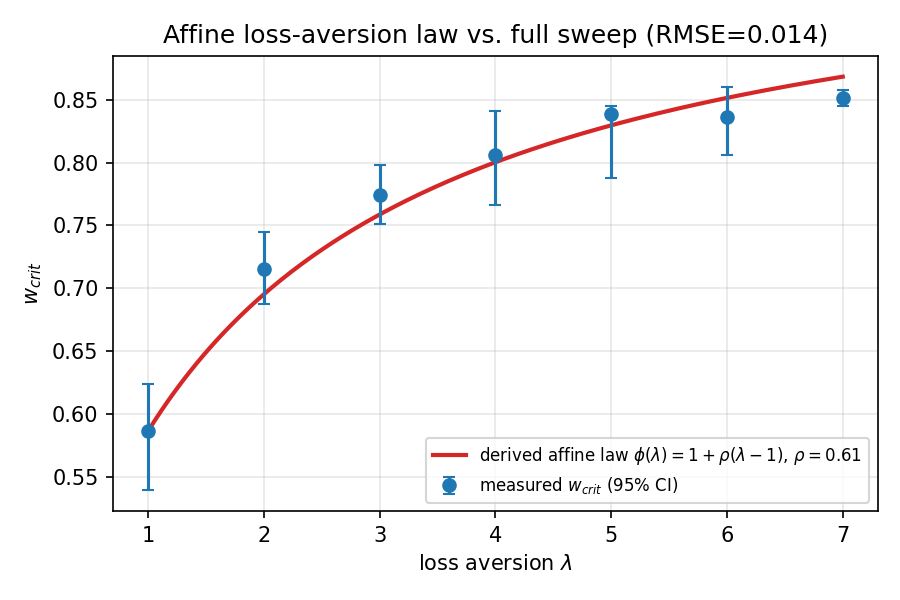
\includegraphics[width=0.82\columnwidth]{Figures/affine_law_7pt}
 \caption{The derived affine law~\eqref{eq:wcrit_lambda} (line, single free parameter
  $\rho=0.61$ set from $\lambda\in\{3,7\}$ with $\gamma$ anchored at $\lambda{=}1$) against the
  measured $\wcrit(\lambda)$ (points, bootstrap 95\% CIs). It tracks all seven points to RMSE
  $0.014$ (the four $\lambda\in\{2,4,5,6\}$ held out), with a mild concave residual at the
  high-$\lambda$ plateau.}
 \label{fig:affine}
\end{figure}

\begin{table}[t]
\centering
\caption{What the mechanism claims. The predictive content is sign and form; the magnitude is
calibrated, and we make no closed-form claim for $\wcrit$.}
\label{tab:ledger}
{\setlength{\tabcolsep}{4pt}\small
\begin{tabular}{@{}lp{0.66\columnwidth}@{}}
\toprule
Derived (no fit) & opposite signs; monotone $\wcrit(\lambda)$; affine $\phi$ with $\rho\in[0,1]$; abrupt sharpness; $\wcrit$ falls with $T$ \\
\addlinespace
Confirmed & opposite signs, affine form; horizon slide (also MPE, LBF); exploration-noise dependence \\
\addlinespace
Calibrated & $\gamma$; loss-domain share $\rho$; noise scale \\
\addlinespace
Not claimed & closed-form $\wcrit$; magnitude on any axis \\
\bottomrule
\end{tabular}}
\end{table}

% =======================================================================
\section{The Instrument Travels; So Does the Direction}
\label{sec:generalization}

The first thing that must generalize is the \emph{instrument}: the pre-registered boundary is only
useful if it can be measured in environments beyond the supply chain. It can: we estimate a
CI'd $\wcrit$ in two further environments and under a second algorithm, and using it there, we ask
whether the behavioral finding travels. The mechanism commits in advance to a direction (loss
aversion biases the drift toward the lazy action, raising $\wcrit$); if that is not an artifact of one substrate or
optimizer, the sign should survive changing both. We match the learner to each environment
(independent PPO where coordination is locally learnable; centralized-critic
MAPPO~\citep{yu2022surprising} where reward is shared-global). The direction is robust in every
setting; the absolute level, curvature sign, and functional form are not
(Figure~\ref{fig:generalization}, Table~\ref{tab:generalization}).
On the \emph{supply chain under MAPPO} (only the learner changes), $\wcrit$ rises $0.796\to0.889$,
monotone from $\lambda{=}2$, converging with PPO by $\lambda\!\geq\!4$. On \emph{MPE} the
loss-aversion excess is $+0.158$ at $\lambda{=}7$ while curvature is null ($+0.042$, CI spans zero);
on \emph{LBF} curvature moves the boundary \emph{right}, and the affine law misfits it by RMSE
$0.15$, both confirming the curvature sign and form are substrate-specific. Thus the
\emph{method}, a CI'd boundary that loss aversion shifts, generalizes across four
environment-algorithm combinations, while the affine constants and curvature sign do not.

\paragraph{Two boundary conditions, both predicted.}
The mechanism makes the boundary contingent on two ingredients, and ablating each confirms it
(Table~\ref{tab:ablation}). \emph{Action representation.} The signal-to-noise crossing is a property
of a continuous gradient, so destroying it should remove the boundary. Value-based learners (QMIX,
IQL) on a discretized $K{=}11$ action space give a flat, $w$-independent collapse rate, but a
single-variable control isolates the cause: PPO on the \emph{same} discrete shell also goes flat, so
it is coarse discretization, not the value-based paradigm, that erases the boundary. This is exactly
the continuous-gradient prediction: coarse bins snap the policy to fixed attractor levels,
suppressing the gradient noise near the boundary so agents never visit the metastable lazy region
where collapse is decided, a scope condition of the mechanism, not a fragility of the method (and
not a claim that discreteness per se removes the boundary: MPE is natively discrete and retains it).
It also scopes whether the loss-aversion direction holds under value-based methods: since those
learners show no measurable boundary here, the question is not well-posed and we claim nothing about
it. \emph{Credit assignment.} On a shared-reward task the boundary is measurable only with a learner
that can coordinate at all: independent PPO collapses at \emph{every} $w$ on MPE (a coordination
floor), while centralized-critic MAPPO recovers it. Each is a confirmed scope condition, not a
negative result.

\begin{table}[t]
\centering
\caption{Action-representation ablation. The control (last row) changes only the action space
while holding the learner at PPO, isolating coarse discretization as what erases the boundary.}
\label{tab:ablation}
{\setlength{\tabcolsep}{5pt}\small
\begin{tabular}{lll}
\toprule
Learner & Action space & Boundary? \\
\midrule
PPO / MAPPO & continuous & yes \\
QMIX (centralized value) & discrete $K{=}11$ & no \\
IQL (independent value) & discrete $K{=}11$ & no \\
PPO (control) & discrete $K{=}11$ & \textbf{no} \\
\bottomrule
\end{tabular}}
\end{table}

\begin{figure}[t]
 \centering
 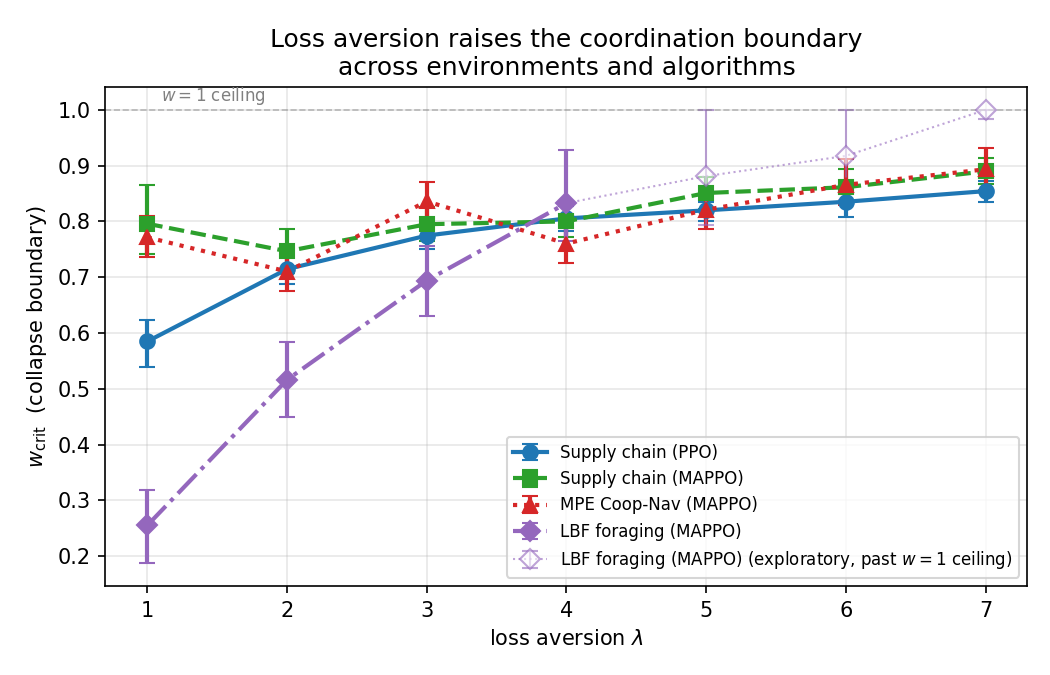
\includegraphics[width=0.95\columnwidth]{Figures/generalization_wcrit_vs_lambda.png}
 \caption{$\wcrit$ versus $\lambda$ across four settings: supply chain under PPO and MAPPO, MPE
  under MAPPO, LBF under MAPPO (bootstrap 95\% CIs). $\wcrit$ rises with $\lambda$ in every
  setting; the \emph{direction} generalizes, while levels (most at $\lambda{=}1$), curvature
  sign, and exact form are substrate-specific. LBF $\lambda{\geq}5$ points extrapolate past the
  $w{=}1$ ceiling (outside the measured grid) and are labeled exploratory.}
 \label{fig:generalization}
\end{figure}

\begin{table}[t]
\centering
\caption{Generalization of the loss-aversion \emph{direction}. The sign holds everywhere; only
the supply chain (PPO) yields the affine law. Detail in the Supplement.}
\label{tab:generalization}
\begin{tabular}{lcc}
\toprule
Setting (algo.) & Loss-av.\ effect & Affine law? \\
\midrule
Supply (PPO)  & $+0.166$ ($\lambda{=}7$) & yes (0.014) \\
Supply (MAPPO) & $0.80\!\to\!0.89$ & -- \\
MPE (MAPPO) & $+0.158$ ($\lambda{=}7$) & no \\
LBF (MAPPO) & $0.26\!\to\!0.83$ & no (0.15) \\
\bottomrule
\end{tabular}
\end{table}

% =======================================================================
\section{A Minority Sets the Boundary}
\label{sec:minority}

The decomposition treats the population as homogeneous, but deployed systems mix loss-averse and
risk-neutral participants. Holding the substrate, PPO config, label, and grid identical to the main
sweep, we ask two questions: how much bias at a critical node is needed to move the boundary, and
which node's bias matters most (Figure~\ref{fig:cascade}).

\paragraph{A single node, dose for dose.}
Sweeping the most downstream node's $\lambda\in\{1,\dots,7\}$ (others risk-neutral) traces a
strictly monotone dose-response: $\wcrit$ rises $0.586\to0.856$, converging on the \emph{fully}
loss-averse value ($0.852$) by $\lambda{=}7$ (Figure~\ref{fig:cascade}b). One node, biased hard
enough, imposes the entire network's requirement, the homogeneous result is the saturation of a
continuous law, not a special case.

\paragraph{Position: proximity to demand, not chain index.}
Placing one $\lambda{=}7$ node at each position, the effect is strongly position-dependent, but the
governing variable is how directly a node's output reaches demand, not a chain index
(Figure~\ref{fig:cascade}a). The two nodes feeding retail directly dominate ($0.856$, $0.800$); the
upstream supplier feeding \emph{only} the dominant downstream node is nearly as strong ($0.797$),
while those \emph{splitting} output across both are weaker ($0.726$, $0.673$). The network is a
branching DAG, not a chain, and $\wcrit$ tracks \emph{path concentration}: a biased node matters
more the more directly and exclusively its product flows to demand, so audit the participant whose
output most directly reaches demand, not the average or merely ``upstream'' one (cf.\ the EGT
tipping-point result of~\citealp{mengesha2025}, here in deep-MARL with a topological signature). The
result is single-substrate \emph{by construction}: ``which node sets the boundary'' is well-posed
only under a directed resource flow, which MPE and LBF lack. We therefore report the cascade as a
\emph{falsifiable prediction, not a tested generalization}, testing it needs a second directed-flow
substrate, and is future work, not an oversight.

\begin{figure}[t]
 \centering
 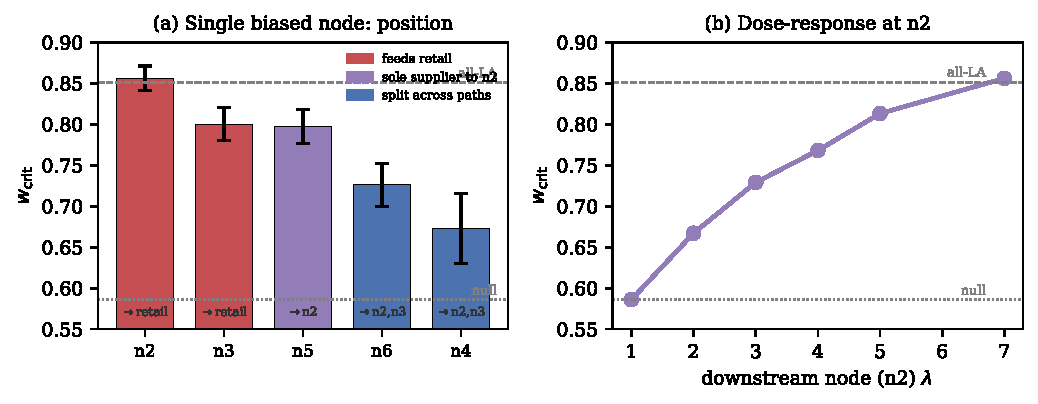
\includegraphics[width=\columnwidth]{Figures/cascade_tier_dose}
 \caption{A minority sets the boundary. (a)~A single $\lambda{=}7$ node by position: nodes feeding
  retail directly (red) dominate; among upstream suppliers, the one feeding \emph{only} the
  dominant downstream node (purple) nearly matches them, while those \emph{splitting} output
  across paths (blue) are weaker, $\wcrit$ tracks path concentration to demand, not chain index.
  (b)~Dose-response: sweeping the downstream node's $\lambda$ traces a strictly monotone rise to
  the homogeneous all-loss-averse value ($0.852$, dashed).}
 \label{fig:cascade}
\end{figure}

% =======================================================================
\section{Discussion}
\label{sec:discussion}

That probability weighting and loss aversion exert opposite effects on the boundary is, to our
knowledge, novel; prior work applies prospect theory as a unified model without decomposing
it~\citep{lalmohammed2025,ghaemi2024risk}. The operational reading is concrete: a system of
$\lambda{=}7$ agents needs $w>0.852$ for reliable coordination against $w>0.685$ for risk-neutral
agents, a $+0.167$ deployment margin that scales with $\lambda$, so domains nearer
$\lambda\!\approx\!2$--$3$ incur a smaller but positive cost. Our phase-diagram framing sits within
a recognized line of multiagent phase-transition
results~\citep{yamaguchi2025,capannoli2026phase} and the broader cooperative-AI
project~\citep{dafoe2020open,hammond2025multiagent,barfuss2020caring}; its distinctive contribution
is a boundary set by the policy-gradient signal-to-noise ratio rather than a fixed update rule.

\paragraph{What a practitioner does with this.}
The boundary is a design quantity: a team can estimate its own $\wcrit$, budget for the
loss-aversion margin rather than discover collapse in production, and (where $w$ is capped) treat
$\lambda$ (set by the training objective~\citep{ethayarajh2024kto,rabin2000risk}) as a second lever.
The minority result adds a targeting rule: audit the biased participant whose output most directly
reaches demand, not the average agent. This targeting is dual-use: the same finding that lets a
defender \emph{harden} the most influential participant equally identifies the node whose induced
bias would most efficiently degrade coordination, which is why we report the decomposition and
cascade openly, so the effect stays auditable rather than hidden.

\paragraph{Scope and Future Work.}
Three boundaries each point to a concrete next step. \emph{(i) From one substrate to many.} The
quantitative core (the $\wcrit(\lambda)$ law and the cascade) is single-substrate by construction:
the direction, boundary, and metastable slide replicate across environments and a second algorithm,
but the magnitudes belong to one simulator and the affine law does not transfer to LBF. Replicating
the cascade on a second directed-flow domain would make it a tested generalization rather than a
prediction. \emph{(ii) From calibrated to predictive.} The mechanism fixes sign and form but not
magnitude; localizing $\wcrit$ from the learning dynamics resisted two pre-registered probes, both
of which track \emph{where the policy sits}, not \emph{where the boundary is} (Supplement). A
localizing observable is the clearest open problem the paper leaves. \emph{(iii) From bracket to
calibration.} Estimating the effective $\lambda$ of preference-aligned agents from behavior would
tie the behavioral axis to the training pipeline. None undercuts the central, replicated claim, each
marks where measurement ends and prediction begins.

% =======================================================================
\section{Conclusion}
\label{sec:conclusion}

We presented a confidence-intervalled diagram of cooperative-MARL coordination
collapse, and used it to show, a priori and across four environment-algorithm combinations, that
loss aversion raises the centralization a team needs to coordinate. Beyond that finding, the
pre-registered protocol is a reusable instrument: any cooperative-MARL study can report \emph{where}
its system collapses, with error bars, rather than asserting that centralization helps. Crucially,
it is \emph{agnostic to the mechanism inducing collapse}: prospect-theoretic bias is only its first
application, and the same measurement applies to reward design, communication, coordination
incentives, or other algorithms, a quantitative alternative to the qualitative descriptions of
coordination collapse the field currently relies on.

% =======================================================================
\section*{Ethical Statement}

This work uses a simulated substrate with no human subjects or personal data. The dual-use reading
of the minority result and the governance implications of raising centralization are discussed
above; substrate-scoped numbers should be re-measured before deployment.

% =======================================================================
\bibliography{references}

\end{document}
